\section{Introduction}
\label{sec:intro}

Automatic Mental Disease\footnote{In this work, we will use 'mental disorder' and 'mental disease' interchangeably} Detection (MDD) is of great practical value and social benefits, because mental disorders can greatly affect sufferers' life quality~\citep{Dreisbach2019systematic}. 
% \KZ{Why from daily life? this is a bit sudden. Maybe just say MDD is important and beneficial.} from data in daily life
Lots of practices~\citep{coppersmith2015adhd,mowery2017understanding} indicate that people's posts on social media, containing sufficient expressions about their feelings and symptoms, can be an informative data source for MDD. 

However, traditional MDD methods \cite{yates2017depression, trotzek2018utilizing} process every post in the user's posting history, which can include many irrelevant or distracting posts. 
% (e.g. negative emotions, symptom descriptions). 
To avoid these noises, some prior works try to extract key posts as detection basis by clustering \cite{zogan2021depressionnet} or semantic similarity \cite{zhang2022psychiatric}, but these heuristics can still introduce erroneous posts, affecting the subsequent MDD results. 

Moreover, comorbidity of several mental disorders is common \cite{ROCA2009Prevalence}. 
For instance, 75\% of depression patients in the surveyed population also suffer from anxiety disorder in their lifetime \cite{Femke2011Comorbidity}. 
However, multi-disease detection is still under-explored, with most existing works focusing on the detection of single common disorder, such as depression \citep{losada2017erisk, lee2021micromodels}. 

\begin{figure}[t]
    \centering
    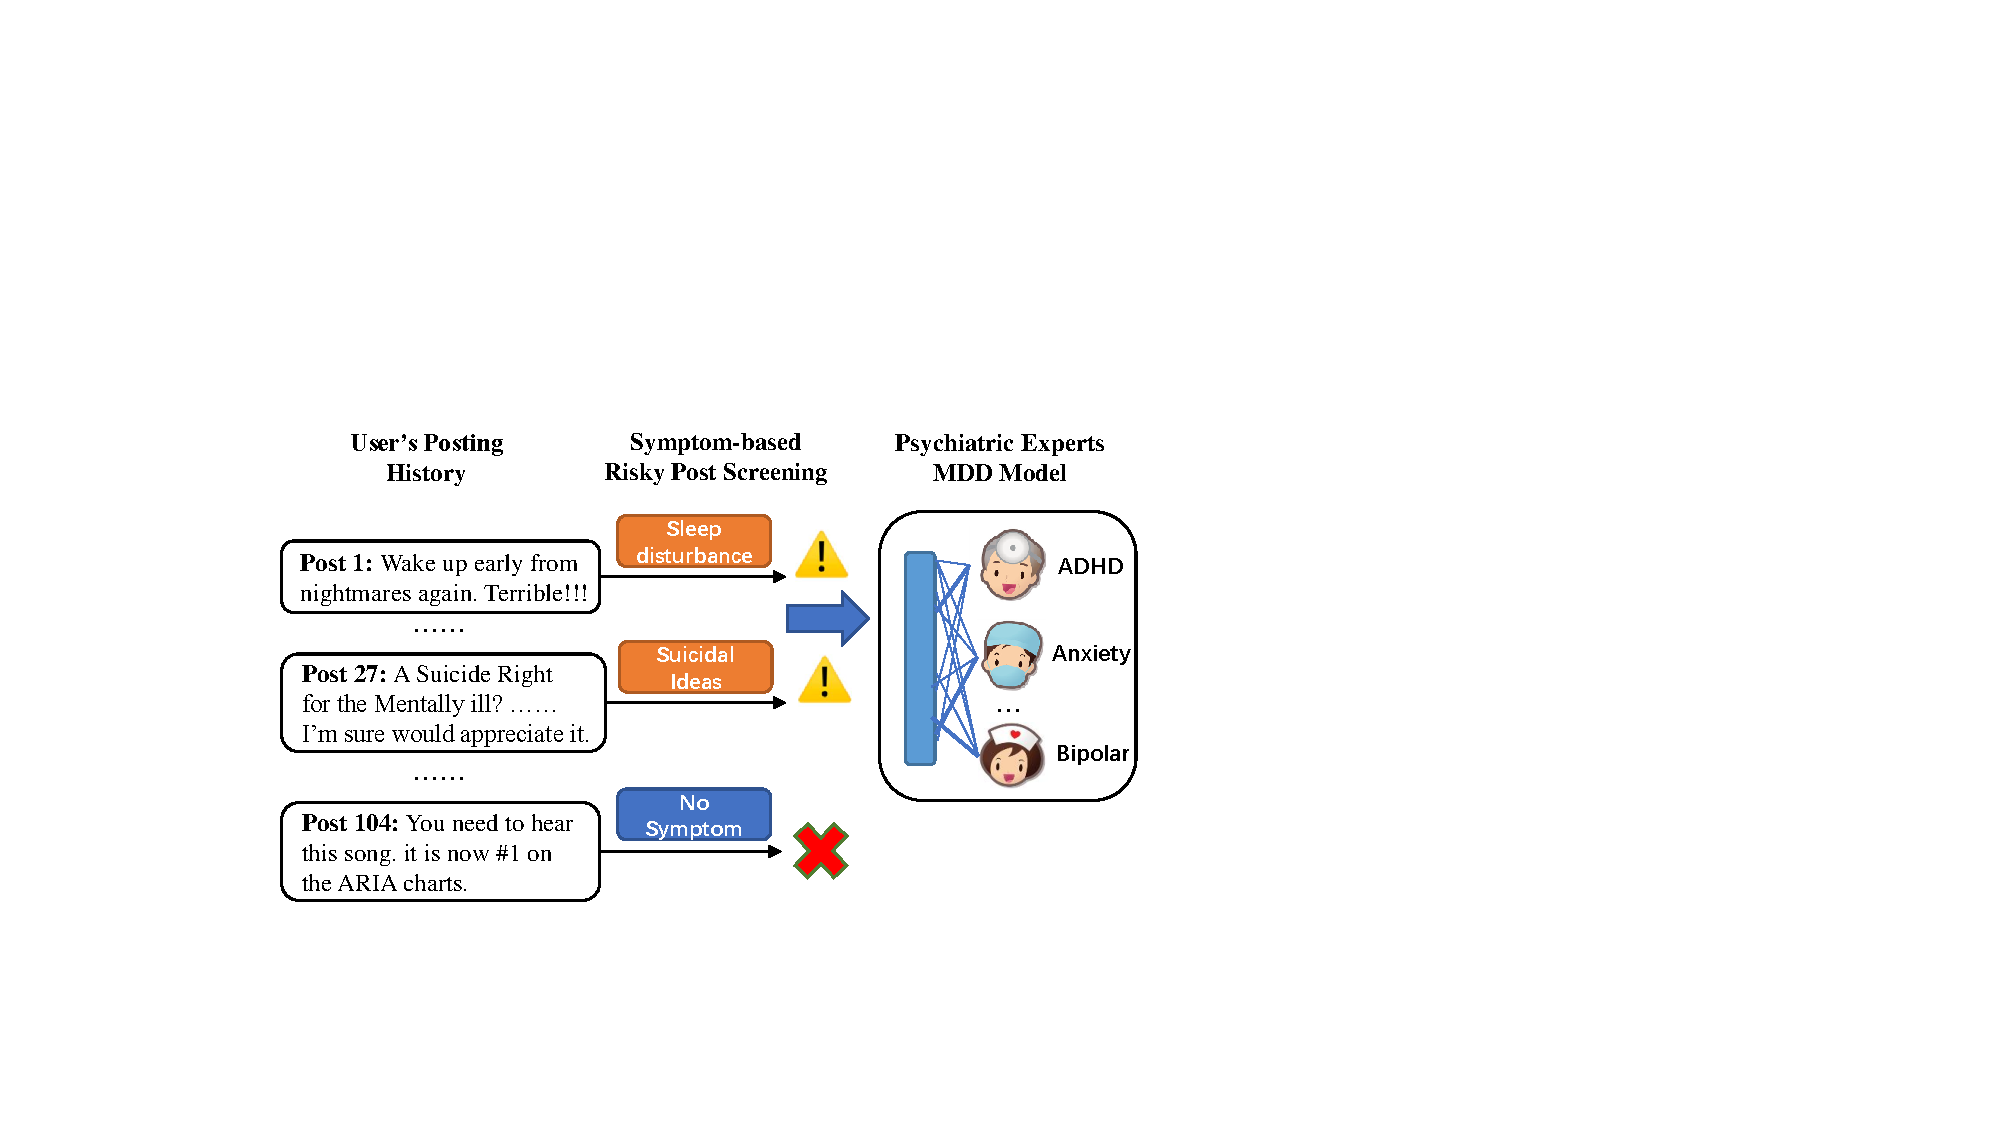
\includegraphics[width=1.0\columnwidth]{figures/pipeline.pdf}
    \caption{Psychiatric Experts Model with Symptom-based Risky Post Screening. Only posts related to symptoms will be selected for further MDD.}
    \label{fig:pipeline}
\end{figure}
% \MYW{according to what stats? cite refs here}


% , by leveraging features like TF-IDF,  LIWC \citep{pennebaker2001linguistic}, or utilizing deep learning methods \citep{yates2017depression, lee2021micromodels}.
% \MYW{Incomplete sentence here}
%myw exisiting models \refs tend to focus on ...single disorder such as well-known xx (give examples, depression)

Comorbidity can be difficult to resolve, as there are lots of overlapping clinical manifestations shared among mental disorders. Pioneering works on multiple disease detection \cite{cohan2018smhd, sekulic2019adapting} commonly yield unsatisfying results as they simply use a shared model architecture for all diseases, which may not be strong enough to distinguish between diseases. \citet{Zhang2022SymptomIF} applies symptom identification for multiple MDD, which can outperform previous pure-text methods due to its better clinical grounding. But it detects each disease separately, ignoring the correlations between them, and thus still gets unsatisfying results on rarer diseases like OCD.

% myw starting like: Few works start to attend for multiple disease detection however commonly yield poor results due to the complexity of the problem and imbalanced data distribution.
%myw you don't have to say black-box nature - your method uses deep learning methods as well. start like: Interpretability is essential in clinical scenarios, however previous methods fail to ..., in particular on those false negative cases. For example, xxx
% myw indeed you need to mention psysym and IJCAI paper here, and your work is on the foundation of them 
% \KZ{You need to say the existing methods are not explainable, give examples.}
%myw different proportion is a weak argument, how about stressing on the entanglement of multiple diseases, e.g. stats in data suggesting #users have multiple diseases, and some are easily confused hence difficult to resolve in a single-disease detection model. This paragraph should state the real challenges and bottleneck of this work, and can relate to your method which is used to tackle these

In this work, we proposed \textbf{PsyEx} (\textbf{Psy}chiatric \textbf{Ex}perts), a novel multi-task learning framework that can simultaneously detect 7 mental disorders\footnote{The 7 mental disorders are: ADHD, Anxiety Disorder, Bipolar Disorder, Depression, Eating Disorder, OCD and PTSD. We place some brief introduction about these disorders in Appendix. \ref{apd:dis_intro}} with a shared backbone and disease-specific structures to leverage the common characteristics of all diseases while still being able to capture their distinctions. 
%myw edit the previous sentence 
First, we only select \textit{risky posts} that are highly relevant to symptoms as interpretable basis for disease detection.
Next, we jointly detect all diseases with a novel model architecture, which has 7 disease-specific psychiatric "experts" on top of a shared hierarchy network, so that the backbone can learn the shared knowledge between diseases, while each expert can focus on their own domain. 
Experiments show that our method can achieve SOTA MDD performance across 7 diseases and bring significant improvement to rarer classes where baselines struggled with. 
Our main contributions are:
\begin{itemize}
    \item We use symptom-based screening to facilitate a precise selection of risky posts.
    \item We propose PsyEx for the better  multi-task learning of 7 mental disorders, which boosts the overall performance by better utilizing the distinctions and commonality among diseases. 
    \item With the interpretability enabled by PsyEx, we further study the contribution of each symptom to the detection of different diseases. 
\end{itemize}
% \MYW{Intro a bit too long}
% Thanks to the recent progress in mental disease symptom identification~\citep{Zhang2022SymptomIF}, we observed that \textit{symptom} can be a promising link between diseases, and provide more interpretability, since many psychiatrists also make a diagnosis based on the symptoms summarized in DSM-5 \cite{american2013diagnostic}. 
%myw this papragraph should better position as "shared knowledge and mixture of experts could help resolve previously-stated challenges", in two ways: disease-individual post selection and MoE modeling. This paragraph and be merged with the next one, stating the proposed method and its significance. 

% In this work, we proposed \textbf{PsyEx} (Psychiatric Experts), a new framework for MDD (Figure.\ref{fig:pipeline}), which simulates the diagnosis decision-making process of psychiatrists. 
% For the user's whole posting history, only posts highly-relevant to symptoms will be selected as \textit{risky posts}, providing interpretable basis for disease detection. 
% Then, we utilize multi-task learning of all diseases with multiple "experts" on top of a shared encoder, so that the backbone can learn the shared knowledge between diseases, while each expert can focus on their own domain. 
% Experiments show that our method can achieve SOTA MDD performance across 7 diseases and bring significant improvement to rarer classes where baselines struggled with. With the interpretability enabled by the multi-expert model and symptom-based risky posts, we can also study the contribution of each symptom to the detection of different diseases. 


